\chapter{Release 3 : Workflow du Budget Non-Industriel (Sprint 4)}
\label{chap:sprint_4}

\section{Introduction}
Les précédents sprints ont permis de maîtriser la capacité de production liée directement au produit automobile (machines de coupe, surface d'assemblage, ressources humaines). Toutefois, le bon fonctionnement d'une usine COFAT dépend également d'un écosystème d'investissements dits «~non-industriels~» : modernisation de l'infrastructure informatique (IT), aménagement des bâtiments (Building), achats logistiques ou encore investissements liés à la qualité (QUALITY). La gestion de ce budget, traditionnellement réalisée par des allers-retours de courriels sans traçabilité ni format unifié, nécessitait une digitalisation urgente.

Ce cinquième chapitre, couvrant le Sprint 4 (Release 3), clôture la réalisation technique du projet. Nous commencerons par définir les objectifs et la complexité technique de ce sprint, en s'appuyant sur les deux modèles Sequelize dédiés. Nous détaillerons ensuite le workflow collaboratif budgétaire implémenté, en insistant sur le rôle volontairement restreint de l'Acheteur (Achat) — confirmé directement par la lecture du code source — et l'absence d'étape de validation formelle par l'Administrateur. Nous expliquerons le mécanisme de notifications asynchrones, la logique de la route \texttt{batch-update} pour les modifications en masse, et les fonctionnalités d'exportation (Excel/PDF) avant d'analyser les interfaces finalisées.

\section{Objectifs et complexité du Sprint 4}
Le développement d'un workflow financier collaboratif au sein d'une SPA (Single Page Application) est techniquement plus ardu que la simple manipulation de données tabulaires. Ce sprint intègre une forte logique d'état partagé entre différents profils d'utilisateurs, une gestion fine des permissions côté serveur, et la génération de fichiers binaires (XLSX, PDF) à la demande.

Les objectifs fixés avec le Product Owner étaient les suivants :
\begin{enumerate}
    \item Permettre la création et la gestion de lignes de budget non-industriel structurées par département.
    \item Implémenter un tunnel de modification stricte des prix par le département Achat, avec recalcul automatique côté serveur via un hook Sequelize.
    \item Assurer une traçabilité des modifications via un système d'alertes (notifications) automatisées et ciblées par rôle.
    \item Générer des rapports professionnels téléchargeables (exports Excel et PDF).
    \item Permettre la mise à jour groupée (batch update) de plusieurs lignes budgétaires en une seule requête HTTP.
\end{enumerate}

\subsection{Modèles de données impliqués}
Pour soutenir ces objectifs, deux modèles Sequelize majeurs ont été implémentés dans la base SQL Server \texttt{GALIA\_V1}. Leur conception reflète les contraintes réelles du métier, sans champ superflu.

\subsubsection{Le modèle \texttt{NonIndustrialBudget}}
C'est le modèle central de ce sprint. Sa définition dans \texttt{models/NonIndustrialBudget.js} révèle les champs suivants (tous vérifiés dans le code source) :
\begin{itemize}
    \item \textbf{\texttt{department} (STRING 50, NOT NULL)} : Le département demandeur. Une validation Sequelize stricte (\texttt{isIn}) contraint les valeurs acceptées à l'ensemble \texttt{['IT', 'HR', 'QUALITY', 'BUILDING', 'LOGISTICS', 'MAINTENANCE', 'PRODUCTION']}. Toute valeur hors de cette liste est rejetée avant même d'atteindre la base de données.
    \item \textbf{\texttt{area} (STRING 100, nullable)} : Le sous-secteur géographique ou fonctionnel au sein du département.
    \item \textbf{\texttt{equipment} (STRING 255, NOT NULL)} : La désignation de l'équipement ou du service à acquérir.
    \item \textbf{\texttt{qty} (INTEGER, NOT NULL, min: 0)} : La quantité demandée, validée pour être positive.
    \item \textbf{\texttt{currency} (STRING 10, default: 'USD')} : La devise de la demande. Les devises supportées dans le frontend sont : TND, USD, EUR, MXN, BRL, EGP.
    \item \textbf{\texttt{unitPrice} (DECIMAL 15,2, NOT NULL, min: 0)} : Le coût unitaire, saisi initialement par le demandeur et modifiable uniquement par l'Acheteur.
    \item \textbf{\texttt{totalPrice} (DECIMAL 15,2, NOT NULL)} : Ce champ n'est \textbf{jamais saisi manuellement}. Il est calculé automatiquement par deux hooks Sequelize : \texttt{beforeValidate} (à la création) et \texttt{beforeUpdate} (lors d'une modification de \texttt{qty} ou \texttt{unitPrice}). La formule est : $totalPrice = qty \times unitPrice$.
    \item \textbf{\texttt{createdBy} (STRING 100)} : Le nom d'utilisateur (username) du Site Manager qui a créé la ligne, utilisé par le système de notifications pour cibler le destinataire.
    \item \textbf{\texttt{updatedBy} (STRING 100)} : Le nom d'utilisateur de la dernière personne ayant modifié la ligne.
\end{itemize}

\textbf{Note d'exactitude technique importante :} Ce modèle ne possède \textbf{pas} de champ \texttt{status}. Il n'existe dans le code source aucun état formel de type « Draft », « Submitted » ou « Approved ». Le workflow n'est pas basé sur une machine à états, mais sur les permissions de rôle appliquées à chaque requête HTTP.

\subsubsection{Le modèle \texttt{BudgetNotification}}
Ce modèle assure la piste d'audit des actions budgétaires. Ses champs réels, issus du fichier \texttt{models/BudgetNotification.js}, sont les suivants :
\begin{itemize}
    \item \textbf{\texttt{type}} : L'événement déclencheur. Les valeurs possibles, définies par une contrainte \texttt{ENUM}, sont : \texttt{NEW\_REQUEST}, \texttt{PRICE\_UPDATED}, \texttt{REQUEST\_MODIFIED}.
    \item \textbf{\texttt{message} (TEXT)} : Le message descriptif de la notification, généré automatiquement par le helper Node.js.
    \item \textbf{\texttt{isRead} (BOOLEAN, default: false)} : Indique si l'utilisateur a consulté la notification.
    \item \textbf{\texttt{budgetItemId} (INTEGER)} : Clé étrangère référençant la ligne de \texttt{NonIndustrialBudget} concernée.
    \item \textbf{\texttt{fromUser} (STRING)} : L'identité de l'acteur ayant déclenché la notification.
    \item \textbf{\texttt{toRole} (STRING)} : Le rôle destinataire de l'alerte ('User', 'Achat', 'Admin').
    \item \textbf{\texttt{toUser} (STRING)} : Le nom d'utilisateur spécifique destinataire (utilisé pour cibler le bon Site Manager).
\end{itemize}

\section{Backlog du Sprint 4}
Le tableau \ref{tab:backlog_sprint4} récapitule les User Stories développées durant ce sprint final. La complexité principale ne résidait pas dans les interfaces graphiques, mais dans la synchronisation des permissions côté serveur Express et dans la logique de ciblage des notifications.

\begin{table}[h]
\centering
\begin{tabular}{|p{1.5cm}|p{8.5cm}|p{2cm}|p{2cm}|}
\hline
\textbf{ID US} & \textbf{Description} & \textbf{Acteur} & \textbf{Complexité} \\ \hline
US-11 & En tant que Site Manager, je veux créer et gérer des lignes de budget avec recalcul automatique du total. & Site Mgr & Moyenne \\ \hline
US-12 & En tant qu'acheteur, je veux modifier le prix unitaire et la devise des demandes existantes. & Achat & Haute \\ \hline
US-13 & En tant qu'utilisateur, je veux voir une cloche de notification se mettre à jour lors d'une action budgétaire. & Tous & Haute \\ \hline
US-14 & En tant qu'admin, je veux exporter le tableau budgétaire au format Excel ou PDF. & Admin & Moyenne \\ \hline
US-15 & En tant qu'acheteur, je veux mettre à jour plusieurs lignes de budget en une seule opération (batch). & Achat & Haute \\ \hline
\end{tabular}
\caption{Backlog spécifique du Sprint 4}
\label{tab:backlog_sprint4}
\end{table}

\section{Le Workflow Budgétaire : Scénario et Permissions}
Le processus métier de demande de budget chez COFAT a été modélisé pour être \textbf{agile et direct}. Contrairement aux lourds systèmes ERP (comme SAP) où chaque étape nécessite l'approbation hiérarchique d'un administrateur, notre système privilégie l'action directe entre le demandeur et le département Achat. \textbf{Il n'y a aucune étape de validation/rejet formelle par l'Administrateur dans ce workflow.}

\subsection{Les étapes du processus}
\begin{table}[h]
\centering
\begin{tabular}{|p{2cm}|p{3.5cm}|p{9.5cm}|}
\hline
\textbf{Étape} & \textbf{Acteur actif} & \textbf{Action métier et réaction du système} \\ \hline
\textbf{1. Création} & Site Manager (Demandeur) & Saisie d'une nouvelle ligne via le formulaire inline. Il indique le \textit{Department} (ex: IT), l'\textit{Area}, l'\textit{Equipment} (ex: Serveur Dell), la \textit{Quantity} et son estimation de prix. Le hook Sequelize \texttt{beforeValidate} calcule instantanément le \texttt{totalPrice}. Le backend génère un événement \texttt{NEW\_REQUEST} notifiant le groupe Achat. \\ \hline
\textbf{2. Consultation} & Acheteur (Achat) & L'Achat se connecte et consulte la liste de toutes les lignes budgétaires via \texttt{GET /api/non-industrial-budget/all}. Il peut filtrer par département (ex: IT) ou faire une recherche textuelle sur l'équipement. \\ \hline
\textbf{3. Édition du Prix} & Acheteur (Achat) & L'Achat modifie \textbf{uniquement le coût unitaire (\texttt{unitPrice}) et la devise (\texttt{currency})} sur les lignes dont il a obtenu un devis fournisseur. \textbf{Le backend recalcule instantanément le \texttt{totalPrice}} via le hook \texttt{beforeUpdate}. Une notification de type \texttt{PRICE\_UPDATED} est envoyée au Site Manager créateur. \\ \hline
\end{tabular}
\caption{Déroulement du workflow du budget non-industriel}
\label{tab:workflow_budget}
\end{table}

\subsection{Implémentation de la sécurité RBAC côté serveur}
La restriction du rôle Achat est strictement implémentée dans le routeur \texttt{routers/nonIndustrialBudgetRoutes.js}. Lors d'une requête \texttt{PUT /update/:id}, le middleware extrait le rôle de l'utilisateur depuis l'en-tête HTTP \texttt{x-user-role}. La logique conditionnelle est la suivante :

\begin{verbatim}
const userRole = req.headers['x-user-role'] || req.body.userRole;
if (userRole === 'Achat') {
  // Achat : modification restreinte à currency et unitPrice uniquement
  if (currency !== undefined) budget.currency = currency;
  if (unitPrice !== undefined) budget.unitPrice = parseFloat(unitPrice);
  if (updatedBy !== undefined) budget.updatedBy = updatedBy;
} else {
  // Autres rôles : modification de tous les champs
  if (area !== undefined) budget.area = area;
  if (equipment !== undefined) budget.equipment = equipment;
  if (qty !== undefined) budget.qty = parseInt(qty);
  if (currency !== undefined) budget.currency = currency;
  if (unitPrice !== undefined) budget.unitPrice = parseFloat(unitPrice);
  if (updatedBy !== undefined) budget.updatedBy = updatedBy;
}
\end{verbatim}

Ce bloc de code garantit que même si le frontend d'un Acheteur malveillant tentait d'envoyer un champ \texttt{qty} ou \texttt{equipment} modifié, le serveur ignorerait silencieusement ces champs. La sécurité est appliquée au niveau de la couche métier (serveur), et non pas uniquement au niveau de l'interface utilisateur.

\subsection{La mise à jour en masse (Batch Update)}
Pour les situations où l'Acheteur doit réviser les prix d'un grand nombre de lignes après une négociation de contrat cadre, l'application propose une route \texttt{PUT /api/non-industrial-budget/batch-update}. Cette route accepte un tableau JSON d'items à mettre à jour :

\begin{verbatim}
{ "items": [ {"id": 12, "unitPrice": 5500, "currency": "EUR"},
             {"id": 17, "unitPrice": 1200, "currency": "USD"} ],
  "updatedBy": "acheteur.central",
  "userRole": "Achat" }
\end{verbatim}

Côté serveur, un \texttt{Promise.all()} parallélise les opérations \texttt{findByPk + save} pour chaque item, en appliquant les mêmes restrictions RBAC que pour la mise à jour unitaire. Cette approche réduit drastiquement le nombre de requêtes HTTP nécessaires pour une mise à jour massive.

\section{Système de Notifications Automatisées}
Pour remplacer les échanges d'emails asynchrones et informels, le système intègre un moteur de notification intra-applicatif. Ce module est implémenté dans \texttt{utils/budgetNotificationHelper.js} et exposé via des routes dédiées sous \texttt{/api/non-industrial-budget/notifications/}.

\subsection{Mécanisme technique de création}
Chaque fois qu'une action budgétaire significative est interceptée par une route Express, une entrée est créée dans la table \texttt{BudgetNotification} avec un ciblage précis :

\begin{itemize}
    \item \textbf{À la création d'une ligne (POST /create)} : Le système appelle \texttt{createBudgetNotification()} avec \texttt{type: 'NEW\_REQUEST'} et \texttt{toRole: 'Achat'}. Tous les acheteurs du groupe sont ainsi alertés d'une nouvelle demande.
    \item \textbf{Quand l'Achat met à jour un prix (PUT /update/:id)} : Une notification \texttt{PRICE\_UPDATED} est créée, ciblée spécifiquement vers \texttt{toRole: 'User'} et \texttt{toUser: budget.createdBy}. Seul le Site Manager auteur de la demande est notifié.
    \item \textbf{Quand un Site Manager modifie sa demande} : Une notification \texttt{REQUEST\_MODIFIED} est envoyée vers \texttt{toRole: 'Achat'}, signalant que les paramètres d'une demande ont changé.
\end{itemize}

\subsection{Consultation des notifications côté client}
Côté client React, une icône «~Cloche~» présente dans la barre de navigation de toutes les pages interroge régulièrement l'API par \textit{polling} (requêtes \texttt{GET} périodiques vers \texttt{/api/non-industrial-budget/notifications/unread}). La requête transmet le rôle de l'utilisateur courant via l'en-tête \texttt{x-user-role}, permettant au serveur de filtrer les notifications pertinentes. Le compteur de notifications non lues (\texttt{isRead: false}) s'affiche sous la forme d'un badge numérique rouge sur la cloche. Au clic, les messages s'affichent dans un panneau déroulant. Une requête \texttt{PUT /notifications/:id/read} marque chaque alerte comme lue dans la base de données. La route \texttt{PUT /notifications/read-all} permet de tout solder en un clic.

\vspace{0.5cm}
\begin{figure}[H]
    \centering
    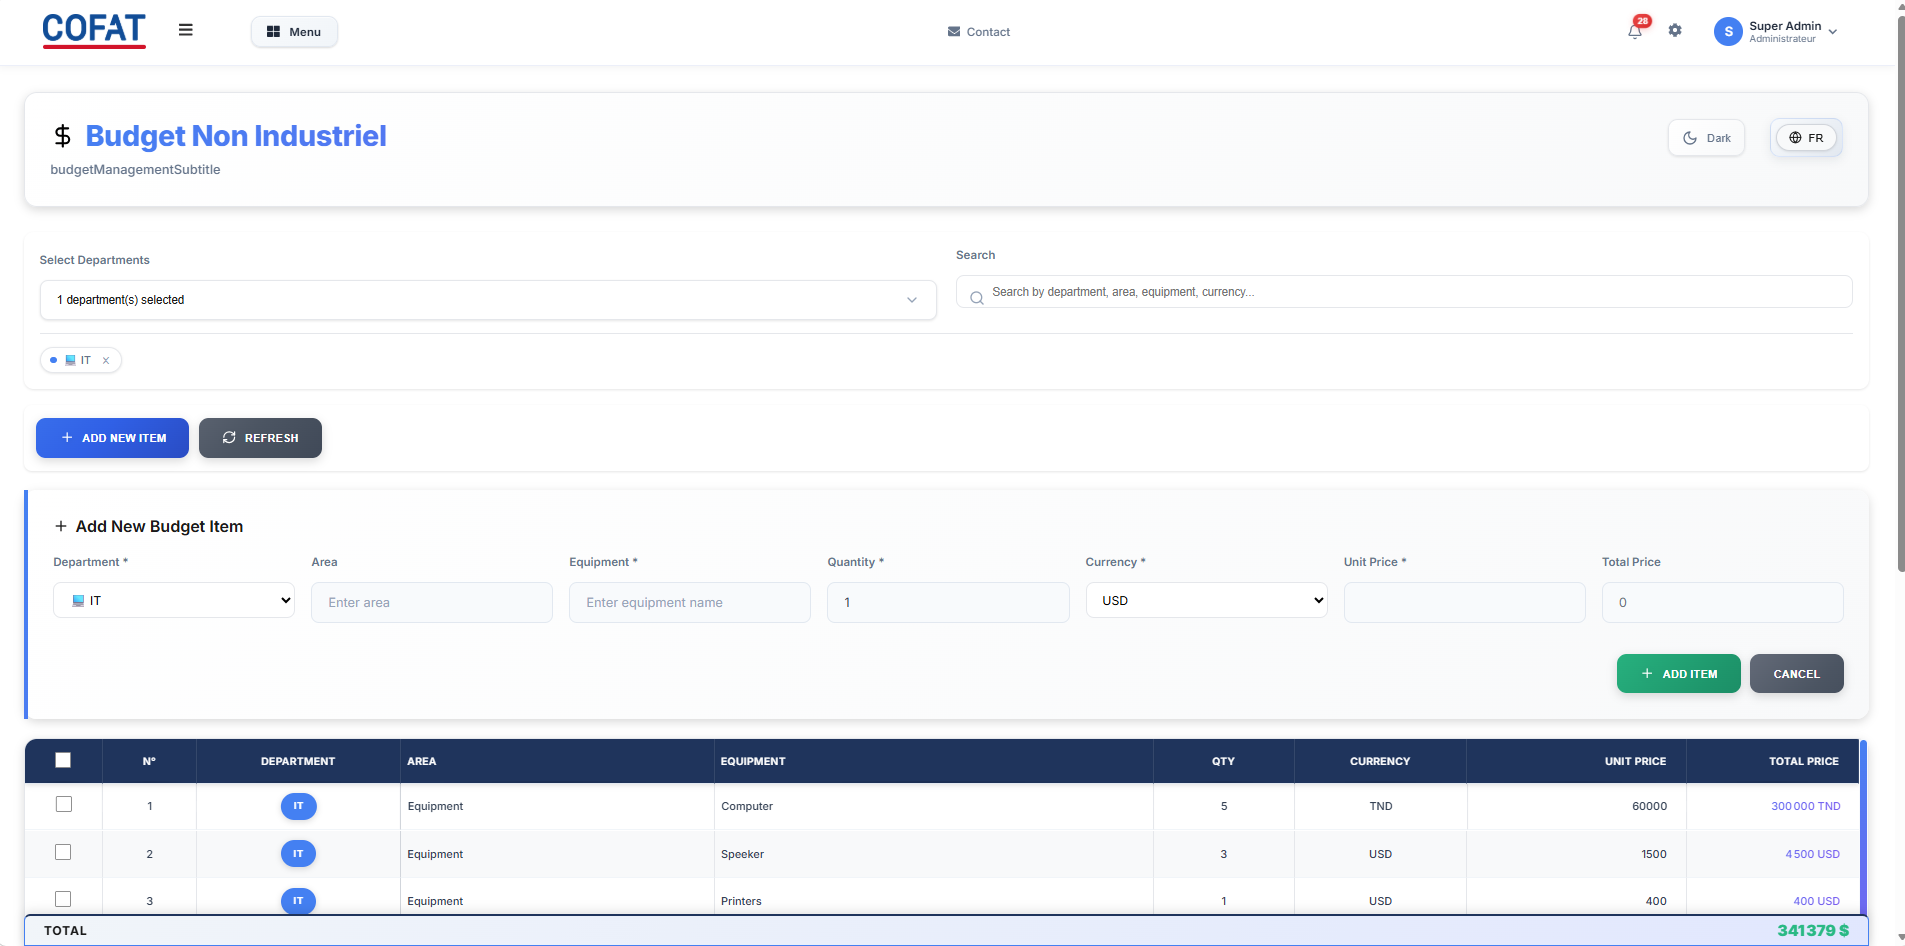
\includegraphics[width=1\textwidth]{img/non industrial budget.png}
    \caption{Interface de gestion dynamique du budget non-industriel}
    \label{fig:non_industrial_budget}
\end{figure}
\vspace{0.5cm}

\section{Exportation (Excel et PDF)}
Lors des réunions du Comité de Direction, le besoin d'extraire la donnée du système pour les présentations officielles est indispensable. L'US-14 a matérialisé les fonctionnalités d'export.

\subsection{Export Excel côté serveur}
Plutôt que de générer le fichier dans le navigateur via React (ce qui peut bloquer le thread principal sur de grands tableaux), l'export est généré intégralement sur le serveur Node.js, garantissant la stabilité de l'application. Le processus, implémenté dans \texttt{utils/excelImporter.js} via la bibliothèque \texttt{xlsx} (SheetJS), se déroule en quatre étapes :

\begin{enumerate}
    \item Sequelize exécute un \texttt{findAll} pour récupérer toutes les lignes du département demandé via \texttt{GET /api/non-industrial-budget/export/:department}.
    \item La bibliothèque \texttt{xlsx} crée un nouveau classeur (\textit{workbook}) en mémoire RAM du serveur.
    \item Une feuille (\textit{worksheet}) est peuplée avec les colonnes exactes : \textbf{N°, Department, Area, Equipment, QTY, Currency, Unit Price, Total Price}, ainsi que les champs d'audit (\texttt{createdBy}, \texttt{updatedBy}).
    \item Le classeur est sérialisé en buffer binaire via \texttt{XLSX.write(workbook, \{ type: 'buffer', bookType: 'xlsx' \})} et streamé au navigateur avec l'en-tête HTTP \texttt{Content-Disposition: attachment; filename="budget\_IT\_[timestamp].xlsx"}, déclenchant le téléchargement automatique.
\end{enumerate}

\subsection{Export PDF}
Une logique similaire est appliquée côté serveur en utilisant des bibliothèques de rendu PDF telles que \texttt{jspdf} et \texttt{jspdf-autotable}, qui permettent de formater les données dans un fichier \texttt{.pdf} présentable, incluant un en-tête COFAT et un horodatage officiel. Ce fichier est directement imprimable pour les réunions de validation de la direction générale.

\subsection{Import Excel des données budgétaires}
À l'inverse, l'application permet également l'import en masse de données budgétaires depuis un fichier Excel. La route \texttt{POST /api/non-industrial-budget/import} utilise le middleware \texttt{multer} pour recevoir le fichier, le sauvegarder temporairement dans \texttt{/Uploads/budget/}, puis appeler la fonction \texttt{importBudgetFromExcel()} qui parse le classeur et insère les lignes validées dans la base de données. Le fichier temporaire est supprimé après traitement.

\section{Analyse de l'interface finalisée}

\textbf{Description de l'interface principale (Figure \ref{fig:non_industrial_budget}) :}
L'écran de budgétisation présente un tableau de données exhaustif et dynamique construit avec la DataGrid de Material UI. Les colonnes affichées correspondent exactement aux champs du modèle : \textbf{N°, DEPARTMENT, AREA, EQUIPMENT, QTY, CURRENCY (TND/USD/EUR/MXN/BRL), UNIT PRICE, TOTAL PRICE}. La particularité de cet écran réside dans son formulaire d'ajout \textit{inline}, permettant de saisir une nouvelle ligne directement au-dessus du tableau sans fenêtre modale intrusive. Des boutons d'action rapides (\textbf{ADD NEW ITEM}, \textbf{REFRESH}, \textbf{EXPORT}) trônent au sommet. Le système calcule et maintient en temps réel la \textbf{ligne de TOTAL cumulatif} visible en bas de la grille.

\vspace{0.5cm}
\begin{figure}[H]
    \centering
    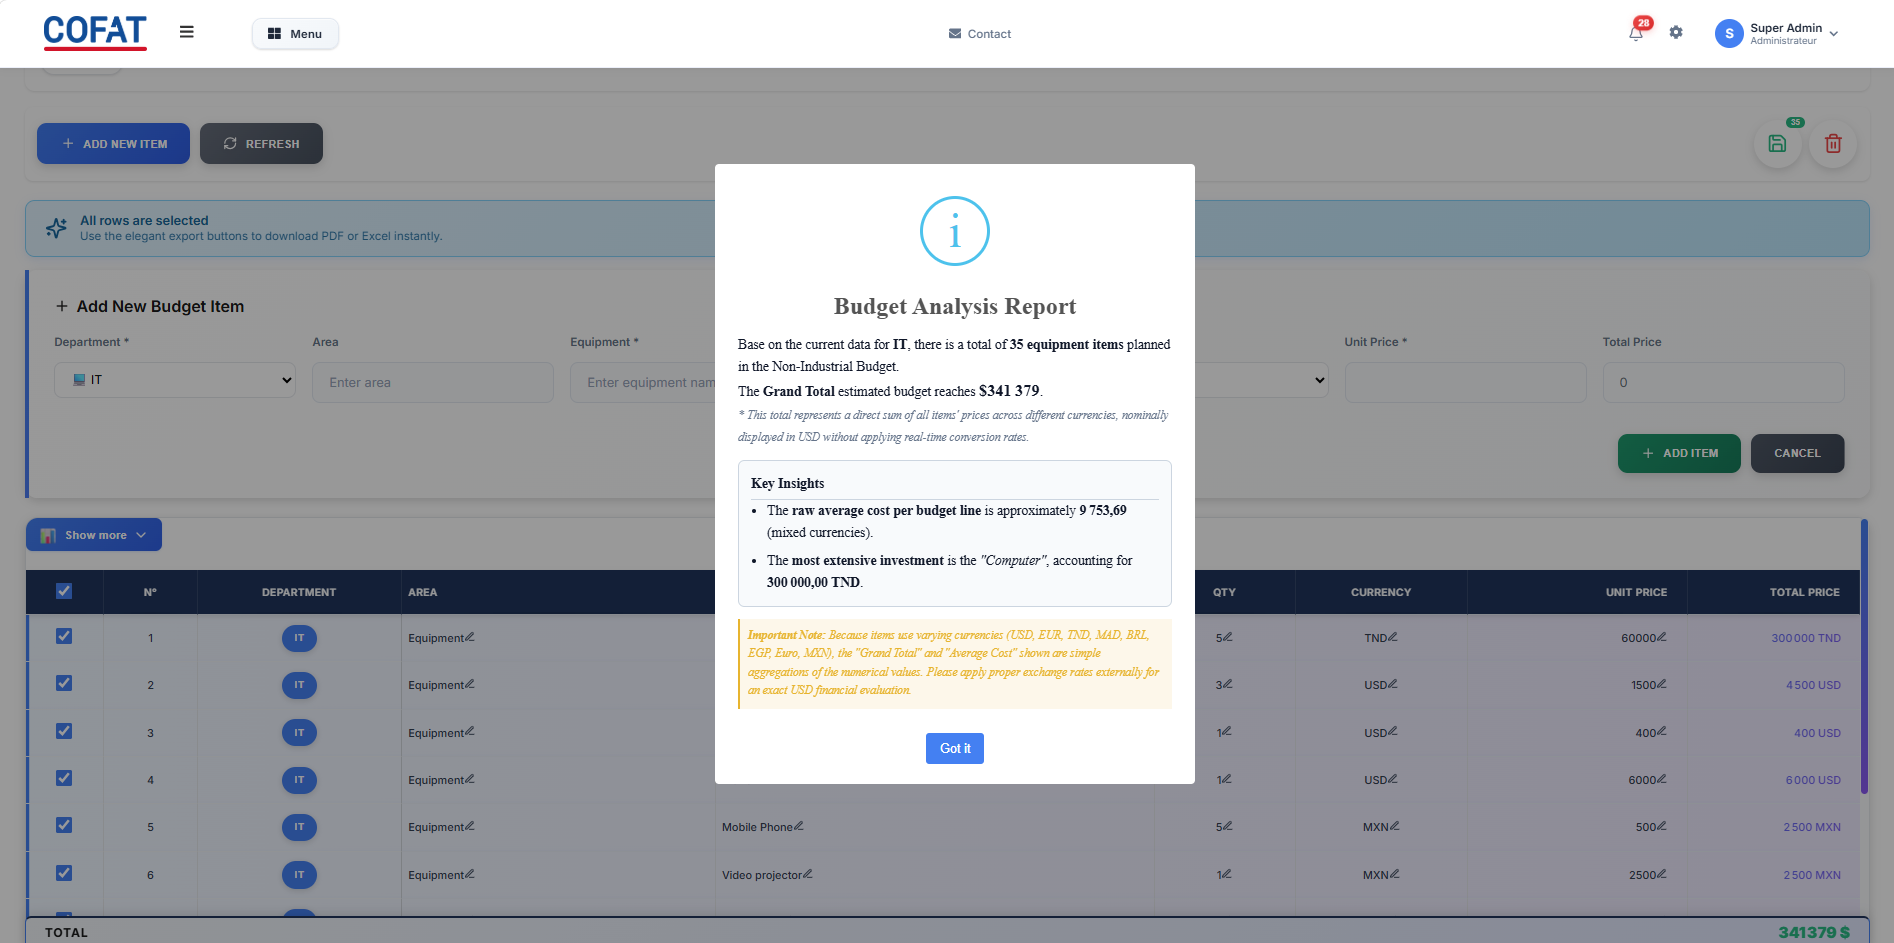
\includegraphics[width=0.9\textwidth]{img/non industrial budget analyse.png}
    \caption{Tableau de bord analytique des dépenses par département}
    \label{fig:analyse_budget}
\end{figure}
\vspace{0.5cm}

\textbf{L'onglet analytique (Figure \ref{fig:analyse_budget}) :}
L'interface propose un onglet analytique dédié aux décideurs. Les graphiques générés par le backend via \texttt{GET /api/non-industrial-budget/stats/by-department} ventilent les dépenses non-industrielles par grand département (IT, Qualité, Bâtiment, Logistique, etc.). Le calcul des statistiques est réalisé côté serveur : Node.js récupère toutes les lignes et applique un \texttt{reduce()} JavaScript pour agréger \texttt{totalAmount}, \texttt{totalItems} et \texttt{totalQty} par département, garantissant une cohérence absolue entre les chiffres affichés et les données de la base SQL Server.

La vue analytique offre ainsi au directeur financier du groupe une vision instantanée, via un graphique en anneau (Doughnut chart) et des histogrammes par devises, de la répartition globale du budget non-industriel.

\section{Conclusion}
Le Sprint 4 a couronné le succès du projet en intégrant la dimension financière à la gestion capacitaire. L'ingénierie du workflow du budget non-industriel prouve la maturité de l'architecture Node.js/React : gestion fine des droits RBAC (restreignant chirurgicalement l'Achat à la modification du coût unitaire et de la devise), recalculs automatiques par les hooks Sequelize (\texttt{beforeValidate}, \texttt{beforeUpdate}), moteur de notification asynchrone ciblé par rôle et par utilisateur, opérations en masse via \texttt{batch-update}, et génération de rapports Excel/PDF côté serveur.

Ces fonctionnalités mettent un terme définitif à la perte de traçabilité et aux lourdeurs bureaucratiques des processus antérieurs basés sur les emails. L'application \textit{Cofat Capacity Study} est désormais complète, opérationnelle, et prête à soutenir la stratégie de croissance globale du Groupe COFAT.
